\section{Why Open Source?}
\AtBeginSection[]
{
	\begin{frame}<beamer>
		\frametitle{Plan}
		\tableofcontents[currentsection]
	\end{frame}
}
\subsection{Rational}



\begin{frame}{Business case \& rational}
	\begin{block}{}
		\begin{itemize}
			\item Context: annual budget reductions
			\item ESRI SDI expensive to run (VFM \& ROI)
			\item Expansion limited due to costs (more cores =\pounds)
			\item The Citrix environment slow making for a poor user experience for those sharing license costs
			 
			\item Too many staff using have access to software with functionality that they do not need
			
			\item Limited funding for training \& lack of  trained Officers 
			
			\item GIS environment is too slow but lack of funding means there is no budget for high specification desktops
			
			
		\end{itemize}
	\end{block}
\end{frame}


\subsection{What we did}
\begin{frame}{What we did}
	\begin{block}{Planning, pilot study \& migration}
		\begin{itemize}
			\item Successful pilot implementation 2013
				\begin{itemize}
					\item PostGIS \& GeoServer set up and QGIS training
					\item 80\%  of testers agreeing that QGIS a viable alternative to ArcView
				\end{itemize}
			\item Decision \- mixed estate
			\item Move ahead with tender \& wider implementation
			
			\item Use savings to pay for training
			
			
			\item Over 70 QGIS users
			
		
			
		\end{itemize}
	\end{block}
\end{frame}


\subsection{How we did it}
\begin{frame}{Data Compatibility}
	\begin{block}{Files and services}
		\begin{itemize}
			\item Shapefile
			\item File GDB
			\item .mdb
			\item WMS (rasters)
			\item PostGIS (with DLLs)
			
			
			\item Spatialite
		
											
		\end{itemize}
			\centering{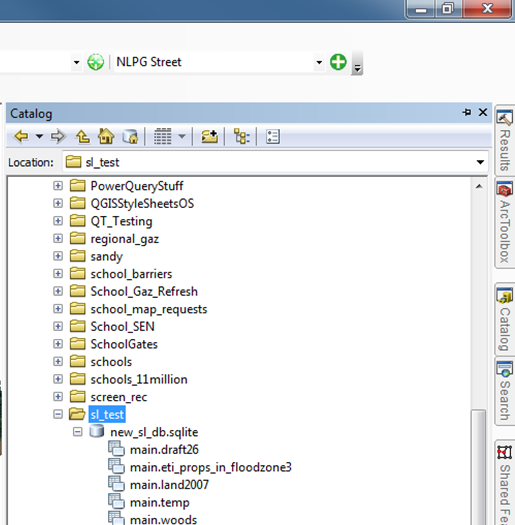
\includegraphics[width=0.25\textwidth]{datacomp.png}}
	\end{block}
\end{frame}


\subsection{Benefits}

\begin{frame}{Benefits}
	\begin{block}{Savings \& benefit}
		\begin{itemize}
			\item Significantly reduced our annual costs 
			\item Promotes collaboration and enables capacity building 
			
			\item Lots of New users
				\begin{itemize}
					\item e.g. Engineers / Flood response Team: 2 ArcView versus 8 QGIS installations
					
				\end{itemize}
						
			\item No vendor lock-in
						
		\end{itemize}
	\end{block}
\end{frame}

\begin{frame}{Benefits}
	\begin{block}{More tools}
		\begin{itemize}
			\item Read/Write multiple data formats (gml)
			 \item Powerful tools - GDAL/OGR
			\item Plug-ins (extensions)
			\begin{itemize}
				\item Hotspot mapping
				
				\item StreetView
				
				\item CrayFish
			\end{itemize}		

						
		\end{itemize}
		\centering{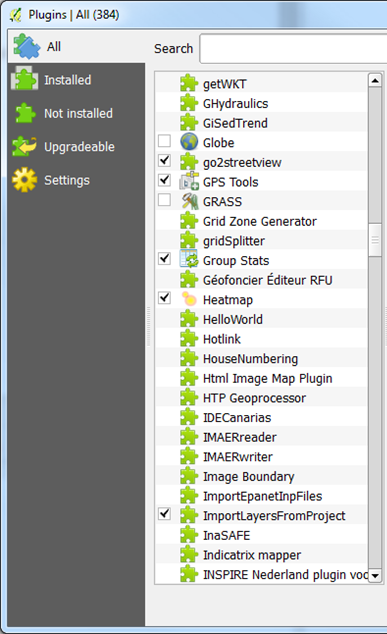
\includegraphics[width=0.25\textwidth]{qgisplugins.png}}
	\end{block}
\end{frame}

\begin{frame}{Benefits}
	\begin{block}{OS MasterMap styling}
	\centering{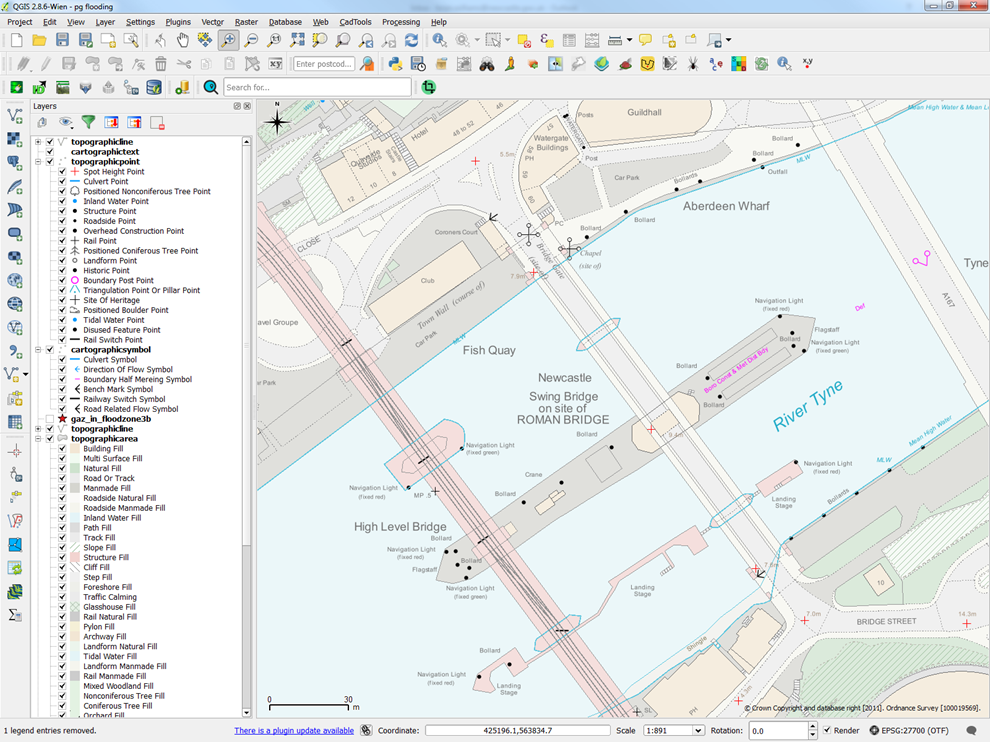
\includegraphics[width=0.8\textwidth]{osmmstyling.png}}
	\end{block}
\end{frame}

\begin{frame}{Benefits}
	\begin{block}{Cool plug-ins}
		\centering{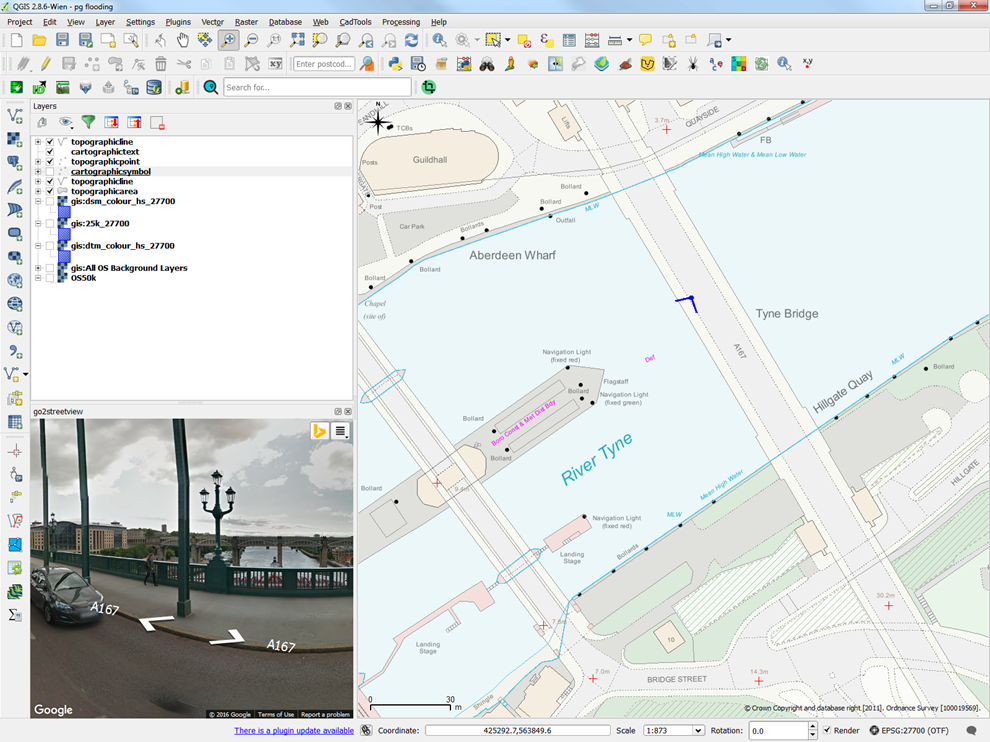
\includegraphics[width=0.8\textwidth]{streetview.png}}
	\end{block}
\end{frame}


\begin{frame}{Benefits}
	\begin{block}{Powerful tools - GDAL/OGR}
		\centering{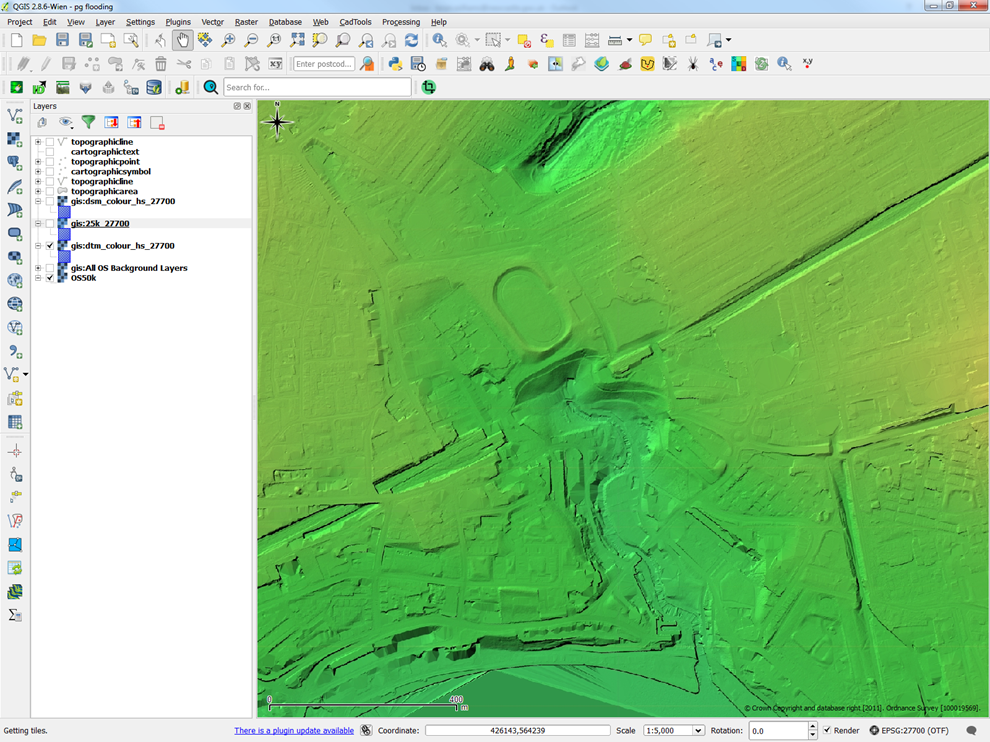
\includegraphics[width=0.8\textwidth]{gdal.png}}
	\end{block}
\end{frame}


\begin{frame}{Benefits}
	\begin{block}{Wider benefits}
		\begin{itemize}
			\item Any code developed by Lutra will be available through an open source type licensing arrangement (GNU General Public License). 
			
			
			\item E.g. Gazetteer Search (Discovery)
	
	\centering{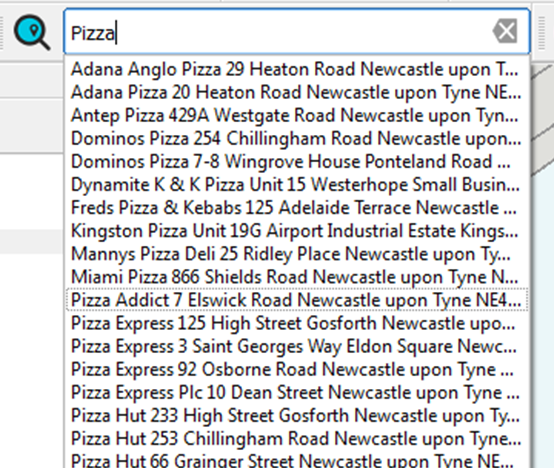
\includegraphics[width=0.3\textwidth]{discovery.png}}
		\end{itemize}
	\end{block}
\end{frame}

\subsection{Discussion Points}
\begin{frame}{Discussion Points}
	\begin{block}{Limitations}
			\begin{itemize}
				\item Functionality available in extensions (Spatial, 3D, Network Analyst)
				
				\item Support for CAD ( DWG is supported)
								
				\item Mobile GIS
							
				\item Advanced editing (e.g. topologies)
				
				\item Advanced cartographic design
				
				
			\end{itemize}
	\end{block}
\end{frame}

\begin{frame}{Discussion Points}
	\begin{block}{Conclusions}
		\begin{itemize}
			\item QGIS and the open source SDI has matured and is a viable alternative to propriety GIS
			
			
			\item Open source does not mean \textbf{'free'}
						
			\item A new business model
			
			
			\item 3rd party Support to reduce risk and provide knowledge
			
			
			\item Opportunities exist to collaborate and share knowledge / code
				\begin{itemize}
					\item  (hence this group)
				\end{itemize}
						
			
		\end{itemize}
	\end{block}
\end{frame}




\section{QGIS}


\begin{frame}{QGIS}
		\begin{block}{Requirement}
			\begin{itemize}
				\item General mapping and analysis
				\item Basic settings and configurations
				\item Print templates
				\item Specific tools and plugins 
				\item Connections to various OGC services
				\item Support and training
			\end{itemize}
		\end{block}
\end{frame}


\subsection{Installer}
\begin{frame}{QGIS installer}

	\centering{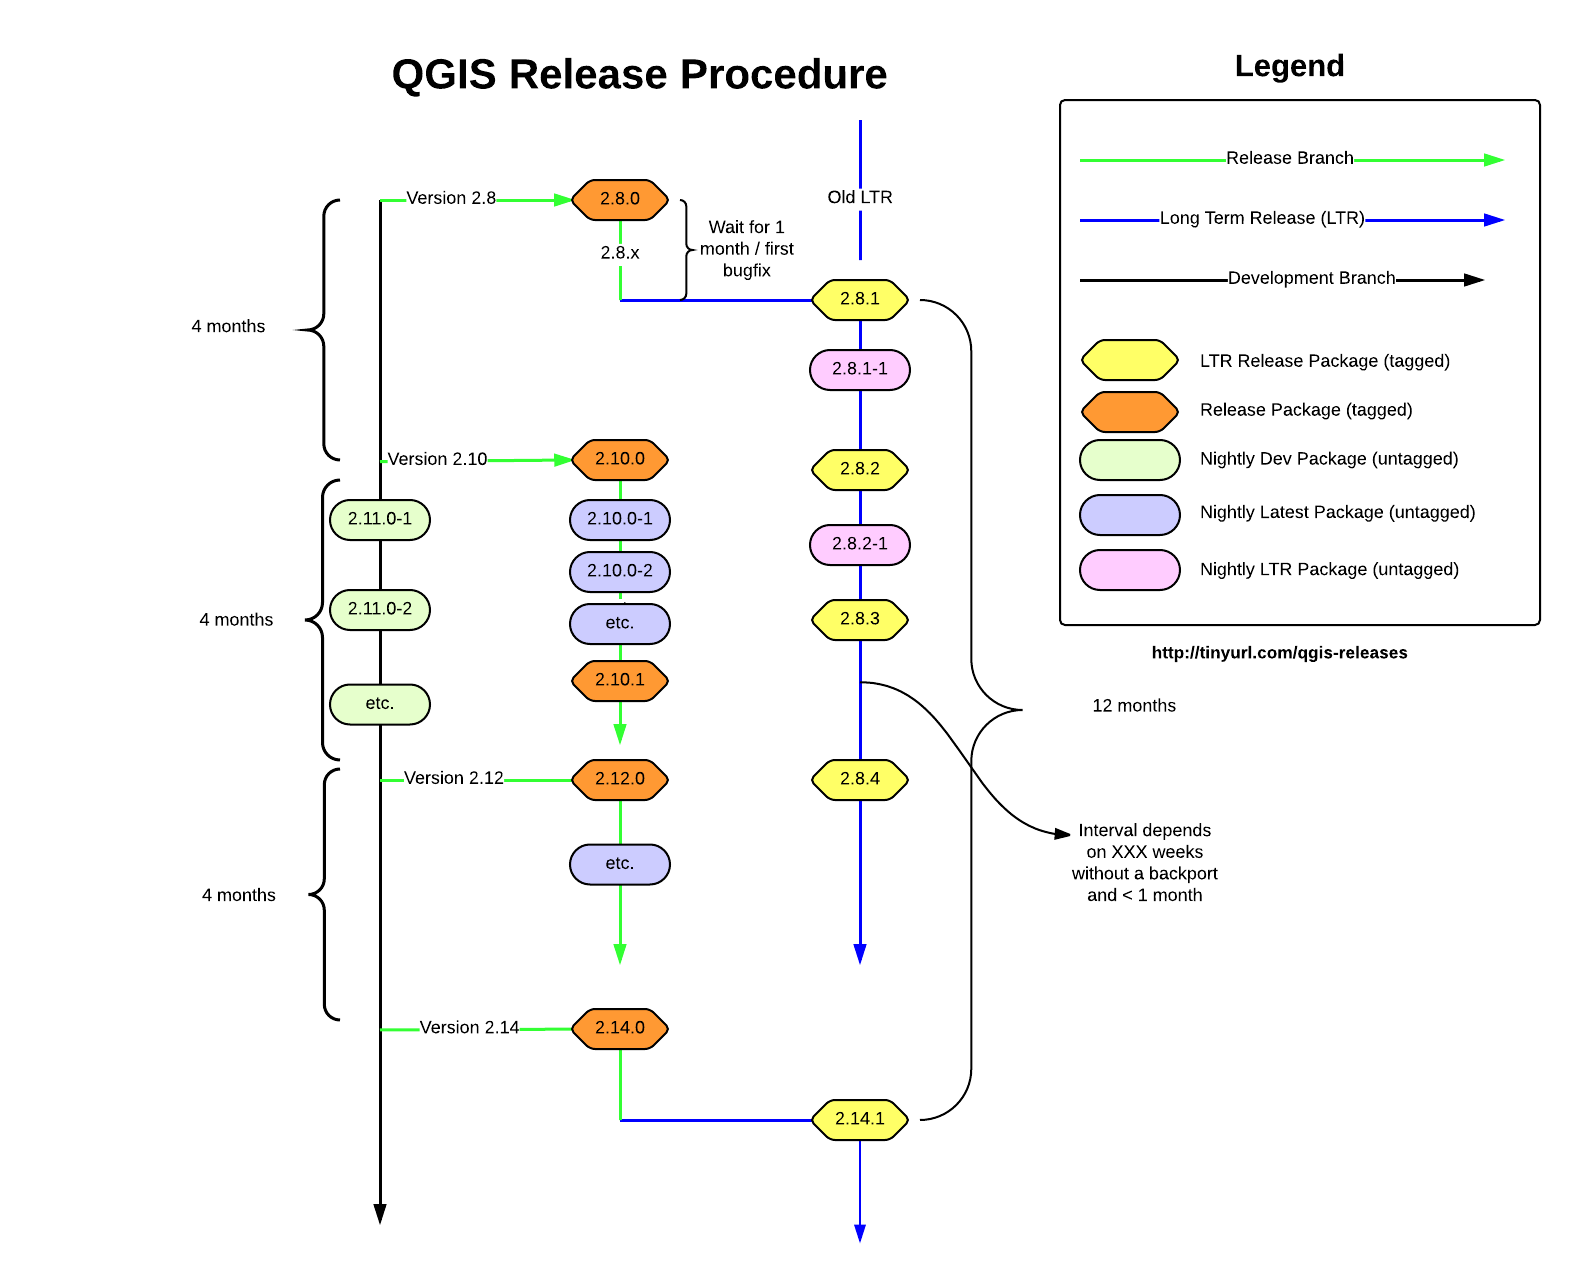
\includegraphics[width=0.9\textwidth]{ae1c0956-523e-11e4-95d9-cea1a3429faf.png}}

\end{frame}


\begin{frame}{QGIS installer}
	
	\centering{\includegraphics[width=0.9\textwidth]{NCCInstaller.png}}
	
\end{frame}

\begin{frame}{QGIS installer}
		\begin{block}{Advantages}
			\begin{itemize}
				\item Reported bugs by the NCC get sorted quicker
				\item Installer is independent of the main QGIS packages
				\item Reported bugs backported to the main QGIS
			\end{itemize}
		\end{block}
	
\end{frame}

\begin{frame}{QGIS installer}
\centering{\includegraphics[width=0.9\textwidth]{SVG-fix.png}}
	
\end{frame}

\begin{frame}{QGIS installer}
	\begin{block}{Customisations}
		\begin{itemize}
			\item Default CRS
			\item Proxy settings
			\item Connection to PostGIS
			\item Connection to WM(T)S
		\end{itemize}
	\end{block}
	
\end{frame}

\begin{frame}{QGIS installer}
	\centering{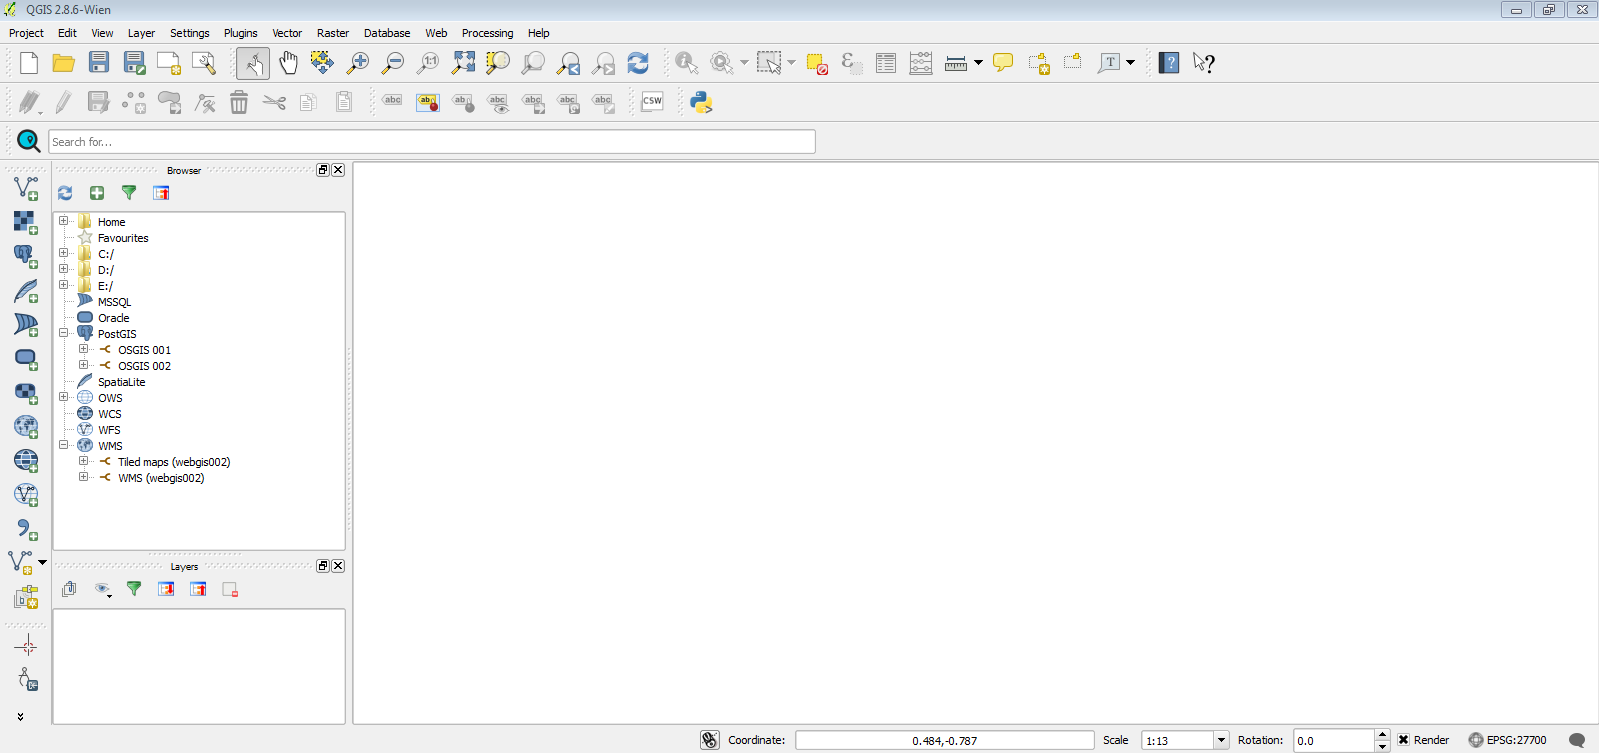
\includegraphics[width=0.9\textwidth]{qgis_ncc.png}}
	
\end{frame}
\begin{frame}{QGIS installer}
	\centering{
\includegraphics[width=0.9\textwidth]{b77ada24-3f76-11e5-808f-6686696e19f0.jpg}}
	
\end{frame}

\subsection{Support}
\begin{frame}{Support}
	\begin{block}{Major bugs resolved}
		\begin{itemize}
			\item Active Directory/user permissions to run Processing
			\item Issue with 32-bit GDB file
		\end{itemize}
	\end{block}
	
\end{frame}

\subsection{Plugins}
\begin{frame}{Plugins}
	\begin{block}{Discovery}
		\begin{itemize}
			\item A QGIS plugin
			\item Using address database from PostGIS
		\end{itemize}
	\end{block}
	
\end{frame}

\begin{frame}{Plugins}
	\begin{block}{Discovery - in action}
\end{block}	
\end{frame}

\subsection{Training}
\begin{frame}{Training}
	\begin{block}{Training for:}
		\begin{itemize}
			\item New to GIS
			\item Existing ESRI users
		\end{itemize}
	\end{block}	
\end{frame}



\section{PostGIS}

\subsection{Migrating data}

\begin{frame}{PostGIS}
	\begin{block}{Migrating data}
		\begin{itemize}
			\item OS Translator II
			\item ogr2ogr scripts
		\end{itemize}
	\end{block}	
\end{frame}

\begin{frame}{PostGIS}
	\begin{block}{Migrating data}
		\begin{itemize}
			\item Test server
			\item Main server
				\begin{itemize}
					\item with back-up / restore script
				\end{itemize}
		\end{itemize}
	\end{block}	
\end{frame}

\subsection{Sync tool with ArcSDE}

\begin{frame}{PostGIS}
	\begin{block}{Sync tool with ArcSDE}
		\begin{itemize}
			\item Waiting for ESRI support (1 year!)
		\end{itemize}
	\end{block}	
\end{frame}

\section{WebGIS and Geoserver}
\begin{frame}{Geoserver}
\centering{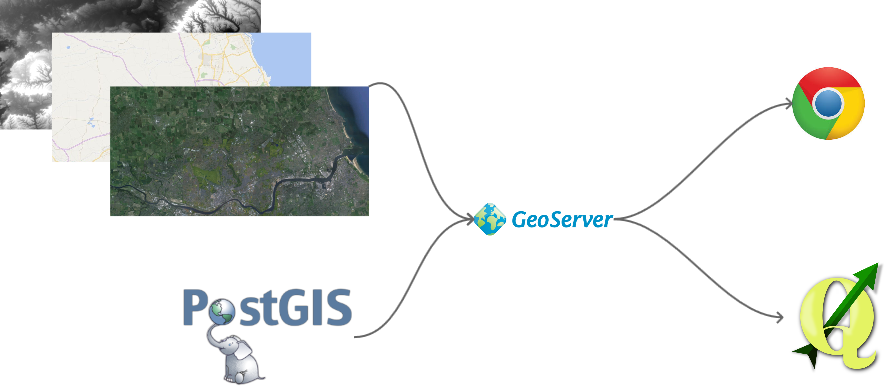
\includegraphics[width=1.0\textwidth]{webgis.png}}
\end{frame}

\begin{frame}{WebGIS}
	\begin{block}{A simple webmap to:}
		\begin{itemize}
			\item Publish select council datasets to the public and council staff
			\item Provide a means for staff to self-serve address data 
		\end{itemize}
	\end{block}	
\end{frame}


\begin{frame}{WebGIS}
	\begin{block}{Key features:}
		\begin{itemize}
			\item Find my nearest tool
			\begin{itemize}
				\item school(s)
				\item customer service
			\end{itemize}	
			\item Gazetteer / search
			\item Produces printable PDF
			\item Download data
		\end{itemize}
	\end{block}	
\end{frame}

\begin{frame}{WebGIS}
	\begin{block}{Implementation:}
		\begin{itemize}
			\item All running on MS Windows
			\item PostGIS
			\item Geoserver + Geoserver Printing module
			\item Bespoke back-end services for
					\begin{itemize}
						\item Find my nearest
						\item Gazetteer
						\item Download
					\end{itemize}
			\item OpenLayers3
		\end{itemize}
	\end{block}	
\end{frame}


